\section{Google Cloud Function}

O Google Cloud Functions se qualifica como uma forma simples de executar código em nuvem, fazendo escalonamento automático com alta tolerância a falhas que dispensa provisionamento e configurações de servidor e oferece cobrança somente quando o o código esta em execução.

\subsection{Propósito}

De acordo com a documentação da Google, os principais propósitos do Cloud Functions são, entregar ao desenvolvedor uma plataforma leve para criar funções independentes que respondam a eventos da nuvem sem necessidade de gerenciar servidores e ambientes de execução.

Os principais tipos de aplicação pensados para funcionar com essa estrutura são, \textit{back-end} de aplicações sem servidor como sites e aplicativos, processamento de dados, arquivos, \textit{streams} e processos de ETL, além de aplicativos inteligentes, como assistentes virtuais, \textit{chatbots}, analise de video, imagens e analise de sentimento.

\subsection{Implantação}
Para a implantação de um novo código para automação, processamento ou outro proposito, deve-se pensar não a nível de sistema, mas de funções isoladas com comportamentos finalidade única e bem estabelecida. 

\bigskip
Cada uma dessas funções ou comportamentos deve ser escrita na linguagem escolhida dentre uma curta lista de opções. 

\bigskip
De acordo com o passo-a-passo da Google, para implantar uma função no Cloud Functions deve-se seguir 5 passos:
\begin{alineas}
	\item Preparação
	\item Criar uma Cloud Function
	\item Escrever o código da função
	\item Testar a função
	\item Escrever o código da função
	\item Observar registros
\end{alineas}

A etapa de preparação que consiste na habilitação de cobrança e permissões no Google não é relevante do ponto de vista de comparação com o nosso projeto, entretanto a partir do segundo item, a relevância passa a existir.
Criar uma Cloud Function é uma etapa de configuração e ao mesmo tempo de implantação da função que será escrita para o ambiente. Essas configurações abrangem um nome para a função, a quantidade máxima de memória que será alocada, um gatilho para a função que pode vir de múltiplos serviços oferecidos pela nuvem do Google, requisições HTTP e HTTPS. Após a execução desses passos a função está no ar e pronta para responder ao gatilho definido.

\bigskip
A proposta principal desse serviço não é ter uma flexibilidade incrível de configurações e nem garantir uma quantidade enorme de recursos para uma função, mas oferecer um meio simples e rápido de implementar uma função e disponibiliza-la para uso sem a necessidade de gerenciar servidores e ambientes de execução.

\subsubsection{Entrada e saída}

O Google Cloud Functions é bastante limitado em relação a interfaces de entrada e saída. Os possíveis meios entradas são pre-estabelecidos e normalmente são serviços da própria nuvem do Google. No contexto do Cloud Functions as entradas são tradas como \textit{triggers} (gatilhos) e elas estão listadas na Fig. \ref{fig:google-cloud-functions-triggers}. Além disso, no caso das saídas, elas estão restritas somente a execuções de procedimentos sem respostas por parte da função ou como única forma de saída através de respostas a requisições HTTP, ou seja, somente funcionam para gatilhos HTTP. 

\bigskip
Além das restrições em relação a interface de entrada e de saída, existem ainda restrições em relação as definições de segurança. Se um desenvolvedor escolhe HTTP como gatilho de entrada por exemplo, ele só pode funcionar através de HTTPS com TLS configurado pela Google, ou seja inviabiliza uso de autenticação \textit{Client Certificate} (certificados do cliente) por exemplo.

\begin{figure}[ht]
	\centering
	\caption{Gatilhos permitidos}
	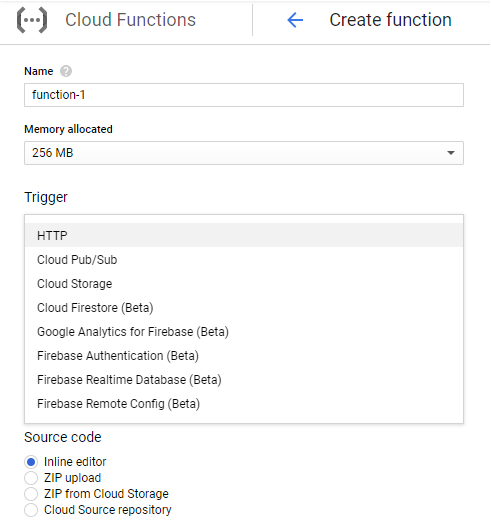
\includegraphics[width=12.5cm]{figuras/google-cloud-functions/triggers.png}
	\legend{Fonte: cloud.google.com/functions/}
	\label{fig:google-cloud-functions-triggers}
\end{figure}


\bigskip
Ou seja, apesar da versatilidade e facilidade de usar Google Cloud Functions, ela vem associada a muitas restrições de entrada e saída e também customizações de segurança.

\subsubsection{Linguagens}

Para os procedimentos e funções rodando no Cloud functions existe uma lista de possíveis linguagens de programação disponíveis, dentre essas linguagens temos Node.js, Python e Go.
Para o Node.js estão disponiveis as versões \textbf{Node.js 6} (deprecada), \textbf{Node.js 8}, \textbf{Node.js 10}, Para Python somente a versão \textbf{Python 3.7.1} e para Go somente \textbf{Go 1.11.65}.

\subsubsection{Escalabilidade}

TODO CONTINUE FROM HERE: https://cloud.google.com/functions/docs/concepts/exec

\subsubsection{Flexibilidade}

TODO

\subsection{Arquitetura}

TODO
\begin{figure}[ht]
	\centering
	\caption{Diagrama de funcionamento}
	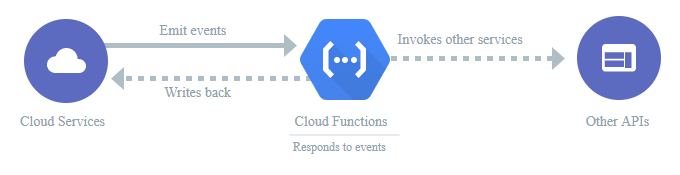
\includegraphics[width=12.5cm]{figuras/google-cloud-functions/workflow.png}
	\legend{Fonte: console.cloud.google.com}
	\label{fig:google-cloud-functions-workflow}
\end{figure}

\subsubsection{Protocolos de rede}

TODO

\subsubsection{Tolerância à falhas}

TODO

\subsection{Licença}

TODO

\subsection{Preço}

TODO

\subsection{Comparação}

TODO
